\let\negmedspace\undefined
\let\negthickspace\undefined
\documentclass[journal,12pt,onecolumn]{IEEEtran}
\usepackage{cite}
\usepackage{amsmath,amssymb,amsfonts,amsthm}
\usepackage{algorithmic}
\usepackage{graphicx}
\usepackage{textcomp}
\usepackage{xcolor}
\usepackage{txfonts}
\usepackage{listings}
\usepackage{enumitem}
\usepackage{mathtools}
\usepackage{gensymb}
\usepackage{comment}
\usepackage[breaklinks=true]{hyperref}
\usepackage{tkz-euclide} 
\usepackage{listings}
\usepackage{gvv}                                        
%\def\inputGnumericTable{}                                 
\usepackage[utf8]{inputenc}

\usepackage{xparse}
\usepackage{color}                                            
\usepackage{array}                                            
\usepackage{longtable}                                       
\usepackage{calc}                                             
\usepackage{multirow}
\usepackage{multicol}
\usepackage{hhline}                                           
\usepackage{ifthen}                                           
\usepackage{lscape}
\usepackage{tabularx}
\usepackage{array}
\usepackage{float}
\newtheorem{theorem}{Theorem}[section]
\newtheorem{problem}{Problem}
\newtheorem{proposition}{Proposition}[section]
\newtheorem{lemma}{Lemma}[section]
\newtheorem{corollary}[theorem]{Corollary}
\newtheorem{example}{Example}[section]
\newtheorem{definition}[problem]{Definition}
\newcommand{\BEQA}{\begin{eqnarray}}
\newcommand{\EEQA}{\end{eqnarray}}
\usepackage{float}
%\newcommand{\define}{\stackrel{\triangle}{=}}
\theoremstyle{remark}
\usepackage{ circuitikz }
\begin{document}

\title{2013 XE}
\author{EE25BTECH11021 - Dhanush sagar}
\maketitle
\renewcommand{\thefigure}{\theenumi}
\renewcommand{\thetable}{\theenumi}

\begin{enumerate}

    \item If $3 \le x \le 5$ and $8 \le y \le 11$ then which of the following options is TRUE? \hfill[GATE 2013 XE]
    \begin{multicols}{2}
    \begin{enumerate}
        \item $\frac{3}{11} \le \frac{x}{y} \le \frac{5}{8}$
        \item $\frac{3}{\brak{11}^2} \le \frac{x}{y} \le \frac{5}{8}$
        \item $\frac{3}{\brak{11}^2} \le \frac{x}{y} \le \frac{5}{\brak{8}^2}$
        \item $\frac{3}{8} \le \frac{x}{y} \le \frac{5}{\brak{8}^2}$
    \end{enumerate}
    \end{multicols}

    \item The Headmaster \underline{\hspace{1.5cm}} to speak to you.  
    Which of the following options is \textbf{incorrect} to complete the above sentence? \hfill[GATE 2013 XE]
    \begin{multicols}{2}
    \begin{enumerate}
        \item is wanting
        \item wants
        \item want
        \item was wanting
    \end{enumerate}
    \end{multicols}

    \item Mahatma Gandhi was known for his humility as \hfill[GATE 2013 XE]
    \begin{multicols}{2}
    \begin{enumerate}
        \item he played an important role in humiliating exit of British from India.
        \item he worked for humanitarian causes.
        \item he displayed modesty in his interactions.
        \item he was a fine human being.
    \end{enumerate}
    \end{multicols}

    \item All engineering students should learn mechanics, mathematics and how to do computation. \hfill[GATE 2013 XE]
    \begin{multicols}{2}
    \begin{enumerate}
        \item mechanics
        \item mathematics
        \item how to do computation
        \item ---
    \end{enumerate}
    \end{multicols}
    Which of the above underlined parts of the sentence is not appropriate?
    \begin{multicols}{2}
    \begin{enumerate}
        \item I
        \item II
        \item III
        \item IV
    \end{enumerate}
    \end{multicols}

    \item Select the pair that best expresses a relationship similar to that expressed in the pair:  
    water : pipe $::$ \hfill[GATE 2013 XE]
    \begin{multicols}{2}
    \begin{enumerate}
        \item cart : road
        \item electricity : wire
        \item sea : beach
        \item music : instrument
    \end{enumerate}
    \end{multicols}
 \item Velocity of an object fired directly in upward direction is given by $v = 80 - 32t$, where $t$ (time) is in seconds. When will the velocity be between $32$ m/sec and $64$ m/sec? \hfill[GATE 2013 XE]
    \begin{multicols}{2}
    \begin{enumerate}
        \item $(1,\,\frac{3}{2})$
        \item $(\frac{1}{2},\,1)$
        \item $(\frac{1}{2},\,\frac{3}{2})$
        \item $(1,\,3)$
    \end{enumerate}
    \end{multicols}

    \item In a factory, two machines M1 and M2 manufacture $60\%$ and $40\%$ of the autocomponents respectively. Out of the total production, $2\%$ of M1 and $3\%$ of M2 are found to be defective. If a randomly drawn autocomponent from the combined lot is found defective, what is the probability that it was manufactured by M2? \hfill[GATE 2013 XE]
    \begin{multicols}{2}
    \begin{enumerate}
        \item $0.35$
        \item $0.45$
        \item $0.5$
        \item $0.4$
    \end{enumerate}
    \end{multicols}

    \item Following table gives data on tourists from different countries visiting India in the year 2011.

\begin{tabular}[12pt]{ |c| c| } 
    \hline
    {Group I: Aircraft mode} & {Group II: Property}\\ 
    \hline
    P: Short period mode & 1: Coupled roll-yaw oscillations\\
    \hline 
    Q: Wing rock & 2: Angle of attack remains constant \\
    \hline
    R: Phugoid mode & 3: Roll oscillations \\
    \hline   
    S: Dutch roll & 4: Speed remains constant\\
    \hline
\end{tabular}


    Which two countries contributed to the one third of the total number of tourists who visited India in 2011? \hfill[GATE 2013 XE]
    \begin{multicols}{2}
    \begin{enumerate}
        \item USA and Japan
        \item USA and Australia
        \item England and France
        \item Japan and Australia
    \end{enumerate}
    \end{multicols}

    \item If $|{-2x}+ 9| = 3$ then the possible value of $|{-x}| - x^{2}$ would be: \hfill[GATE 2013 XE]
    \begin{multicols}{2}
    \begin{enumerate}
        \item $30$
        \item $-30$
        \item $-42$
        \item $42$
    \end{enumerate}
    \end{multicols}

    \item All professors are researchers\\
    Some scientists are professors\\
    Which of the given conclusions is logically valid and is inferred from the above arguments: \hfill[GATE 2013 XE]
    \begin{multicols}{2}
    \begin{enumerate}
        \item All scientists are researchers
        \item All professors are scientists
        \item Some researchers are scientists
        \item No conclusion follows
    \end{enumerate}
    \end{multicols}
    \item The value of the integral 
$$
\int_0^{\infty} e^{-x^2} dx
$$ 
is \\ \hfill[GATE 2013 XE]

\begin{multicols}{4}
\begin{enumerate}
\item $\frac{\sqrt{\pi}}{2}$ 
\item $\sqrt{\pi}$ 
\item $-\sqrt{\pi}$ 
\item $-\frac{\sqrt{\pi}}{2}$
\end{enumerate}
\end{multicols}

\item Which one of the following partial differential equations \textbf{CANNOT} be reduced to two ordinary differential equations by the method of separation of variables? \\ \hfill[GATE 2013 XE]

\begin{multicols}{4}
\begin{enumerate}
\item 
$
\frac{\partial^2 u}{\partial x^2} - \frac{\partial^2 u}{\partial y^2} = 0$
\item 
$
\frac{\partial^2 u}{\partial x^2} - \frac{\partial^2 u}{\partial t^2} = 0
$
\item 
$
\frac{\partial^2 u}{\partial x^2} + \frac{\partial^2 u}{\partial y^2} + \frac{\partial u}{\partial t} = 0
$
\item 
$
\frac{\partial^2 u}{\partial x^2} + \frac{\partial^2 u}{\partial y^2} + \frac{\partial^2 u}{\partial t^2} = 0
$
\end{enumerate}
\end{multicols}

\item The Fourier series of the periodic function 
\begin{align}
    f(x) = |x|, \quad -1 < x < 1, \quad f(x+2) = f(x), \quad x \in \mathbb{R}
\end{align}
is given by 
\begin{align}
\frac{1}{2} - \sum_{n=1}^\infty \frac{4 \cos((2n-1) \pi x)}{(2n-1)^2 \pi^2}.
\end{align}
Using the above, the sum of the infinite series 
\begin{align}
1 + \frac{1}{3^2} + \frac{1}{5^2} + \cdots
\end{align}
is  \hfill[GATE 2013 XE]

\begin{multicols}{4}
\begin{enumerate}
\item $\frac{\pi^2}{4}$
\item $\frac{\pi^2}{8}$
\item $\frac{\pi^2}{6}$
\item $\frac{\pi^2}{2}$
\end{enumerate}
\end{multicols}

\item Consider the function 
$
f(z) = |z|, \quad z \in \mathbb{C}.
$
At $z=0$, the function $f$  \hfill[GATE 2013 XE]

\begin{multicols}{2}
\begin{enumerate}
\item does not satisfy the Cauchy-Riemann equations
\item satisfies the Cauchy-Riemann equations but is not differentiable
\item is differentiable but not analytic
\item is analytic
\end{enumerate}
\end{multicols}

\item The integral 
$
\oint_C \frac{(z+4)}{(z-1)(z-2)^3} dz
$
alng the contour 
$
C: |z - (1 + i)| = 2,
$
oriented anti-clockwise, is equal to  \hfill[GATE 2013 XE]
\begin{multicols}{4}
\begin{enumerate}
\item $0$
\item $\frac{\pi}{e}$
\item $-\frac{\pi}{e}$
\item $\frac{\pi}{i}$
\end{enumerate}
\end{multicols}
\item The integral 
\begin{align}
    \int \int_D y e^{xy} dx dy
\end{align}
over the domain \(D: 0 \leq x \leq 1, 0 \leq y \leq 1\) equals \hfill[GATE 2013 XE]

\begin{multicols}{4}
\begin{enumerate}
\item \(\frac{e-2}{e}\) 
\item \(\frac{e+2}{e}\) 
\item \(\frac{e-1}{e}\) 
\item \(\frac{1-e}{e}\)
\end{enumerate}
\end{multicols}

\item If the mean and variance of a binomial distribution are 6 and 2 respectively, then the probability of two failures is \hfill[GATE 2013 XE]

\begin{multicols}{4}
\begin{enumerate}

\item $4 \brak{\frac{2}{3}}^{7}$
    \item $4 \brak{\frac{2^{2}}{3^{7}}}$
    \item $17 \brak{\frac{2}{3}}^{7}$
    \item $17 \brak{\frac{2^{2}}{3^{7}}}$
\end{enumerate}
\end{multicols}
\item For the matrix $M = \myvec{1 & 0 & -1 \\ 0 & 1 & -1 \\ 1 & 1 & -2}$, consider the following statements:\hfill[GATE 2013 XE]

\begin{itemize}
    \item[(P)] The characteristic equation of $M$ is $\lambda^{3} - \lambda = 0$.
    \item[(Q)] $M^{-1}$ does not exist.
    \item[(R)] The matrix $M$ is diagonalizable.
\end{itemize}

Which of the above statements are true?

\begin{multicols}{2}
\begin{enumerate}
    \item P, Q and R
    \item P and R but not Q
    \item P and Q but not R
    \item Q and R but not P
\end{enumerate}
\end{multicols}
\item The work done by the force
$
\vec{F} = (x + y) \hat{i} + (xy + x) \hat{j}
$
in moving a particle once along the triangle with vertices $(0,0), (1,0)$ and $(0,1)$ in the anti-clockwise direction is \ \hfill[GATE 2013 XE]

\begin{multicols}{4}
\begin{enumerate}
\item 0
\item $\frac{1}{6}$
\item $\frac{1}{3}$
\item $\frac{5}{3}$
\end{enumerate}
\end{multicols}

\item The general solution of the differential equation
\begin{align}
x^2 \frac{d^3 y}{dx^3} + x \frac{d^2 y}{dx^2} + (x - 1)y = 0, 
\end{align}
is  \hfill[GATE 2013 XE]

\begin{multicols}{2}
\begin{enumerate}
\item $C_{1}e^{x}+e^{x/2}\!\left\{\,C_{2}\cos\brak{\tfrac{\sqrt{3}}{2}x}+C_{3}\sin\brak{\tfrac{\sqrt{3}}{2}x}\,\right\}$
    \item $C_{1}x+x^{-1/2}\!\left\{\,C_{2}\cos\brak{\tfrac{\sqrt{3}}{2}\log_{e}x}+C_{3}\sin\brak{\tfrac{\sqrt{3}}{2}\log_{e}x}\,\right\}$
    \item $C_{1}e^{x}+e^{-x/2}\!\left\{\,C_{2}\cos\brak{\tfrac{\sqrt{3}}{2}x}+C_{3}\sin\brak{\tfrac{\sqrt{3}}{2}x}\,\right\}$
    \item $C_{1}x+x^{1/2}\!\left\{\,C_{2}\cos\brak{\tfrac{\sqrt{3}}{2}\log_{e}x}+C_{3}\sin\brak{\tfrac{\sqrt{3}}{2}\log_{e}x}\,\right\}$
\end{enumerate}
\end{multicols}

\item Using Euler’s method to solve the differential equation

$
\frac{dy}{dx} = 2 \cos x, \quad y(0) = 1,
$
with step-size $h=0.25$, the value of $y(0.5)$ is  \hfill[GATE 2013 XE]

\begin{multicols}{4}
\begin{enumerate}
\item 1.3125
\item 1.1875
\item 1.125
\item 1.0625
\end{enumerate}
\end{multicols}
\item The gauge pressure inside a soap bubble of radius $R$, with $\sigma$ denoting the surface tension between the soap solution and air, is: \hfill[GATE 2013 XE]
\begin{multicols}{2}
\begin{enumerate}
    \item $\frac{4\sigma}{R}$
    \item $\frac{2\sigma}{R}$
    \item $\frac{\sigma}{R}$
    \item $\frac{8\sigma}{R}$
\end{enumerate}
\end{multicols}

\item Let $M$, $B$ and $G$ represent respectively the metacentre, centre of buoyancy and the centre of mass of a floating buoy. Which of the following statements is correct? \hfill[GATE 2013 XE]
\begin{multicols}{2}
\begin{enumerate}
    \item $M$ is above $G$; Buoy unstable
    \item $B$ is above $G$; Buoy stable
    \item $M$ is above $G$; Buoy stable
    \item $B$ is above $G$; Buoy unstable
\end{enumerate}
\end{multicols}

\item A reservoir connected to a pipeline is being filled with water, as shown in the figure. At any time $t$, the free surface level in the reservoir is $h$. Find the time in seconds for the reservoir to get filled up to a height of $1\,\mathrm{m}$, if the initial level is $0.2\,\mathrm{m}$ \underline{\hspace{2cm}}. \hfill[GATE 2013 XE] 
\begin{figure}[H]
    \centering
    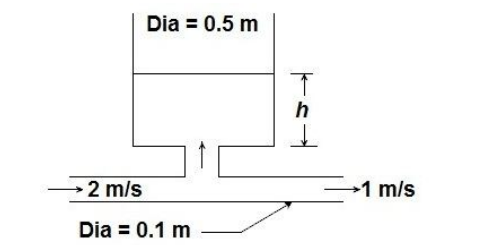
\includegraphics[width=0.5\columnwidth]{figs/fig1.png}
    \caption{}
    \label{fig:fig1}
\end{figure}
\item  Bernoulli’s equation is valid for the following type of flow:
\begin{multicols}{2}
\begin{enumerate}
    \item Compressible, steady, inviscid
    \item Incompressible, steady, viscous
    \item Compressible, unsteady, viscous
    \item Incompressible, steady, inviscid
\end{enumerate}
\end{multicols}

\item If $A$ is the area of a circle of radius $r$ enclosing a plane forced vortex flow, with origin at the centre of the vortex and if $\omega$ is the angular velocity, $\zeta$ is the vorticity, $\vec{V}$ is the velocity vector, then the circulation around the contour of the circle is given by: \hfill[GATE 2013 XE]
\begin{multicols}{2}
\begin{enumerate}
    \item $2\omega A$
    \item $2\zeta A$
    \item $2V A$
    \item $0$
\end{enumerate}
\end{multicols}

\item Flow past a circular cylinder can be produced by superposition of the following elementary potential flows: \hfill[GATE 2013 XE]
\begin{multicols}{2}
\begin{enumerate}
    \item Uniform flow, doublet
    \item Uniform flow, vortex
    \item Source, vortex
    \item Sink, vortex
\end{enumerate}
\end{multicols}

\item Let $\delta$, $\delta_1$ and $\delta_2$ denote respectively the boundary-layer thickness, displacement thickness and the momentum thickness for laminar boundary layer flow of an incompressible fluid over a flat plate. The correct relation among these quantities is: \hfill[GATE 2013 XE]
\begin{multicols}{2}
\begin{enumerate}
    \item $\delta < \delta_1 < \delta_2$
    \item $\delta > \delta_1 > \delta_2$
    \item $\delta > \delta_1 < \delta_2$
    \item $\delta < \delta_1 > \delta_2$
\end{enumerate}
\end{multicols}

\item In the hydrodynamic entry region of a circular duct, the pressure forces balance the sum of: \hfill[GATE 2013 XE]
\begin{multicols}{2}
\begin{enumerate}
    \item viscous and buoyancy forces
    \item inertia and buoyancy forces
    \item inertia and surface tension forces
    \item inertia and viscous forces
\end{enumerate}
\end{multicols}

\item Bodies with various cross-sectional shapes subjected to cross-flow of air are shown in the figures. The characteristic dimension of all the shapes is the same. The cross-sectional shape with the largest coefficient of drag (i.e., sum of the pressure and skin-friction drags), at any moderately large Reynolds number, is: \hfill[GATE 2013 XE]
\begin{figure}[H]
    \centering
    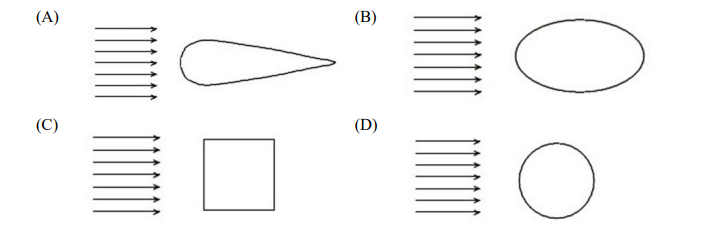
\includegraphics[width=0.5\columnwidth]{figs/fig2.png}
    \caption{}
    \label{fig:fig2}
\end{figure}

\item A U-tube of very small bore, with its limbs in a vertical plane and filled with a liquid of density $\rho$, up to height $h$, is rotated about a vertical axis, with angular velocity $\omega$, as shown in the figure. The radius of each limb from the axis of rotation is $R$. Let $p_a$ be the atmospheric pressure and $g$ the acceleration due to gravity. The angular velocity at which the pressure at the point $O$ becomes half of the atmospheric pressure is given by: \hfill[GATE 2013 XE]

\begin{figure}[H]
    \centering
    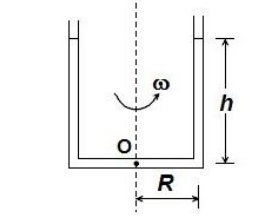
\includegraphics[width=0.5\columnwidth]{figs/fig3.png}
    \caption{}
    \label{fig:fig3}
\end{figure}
\begin{multicols}{4}
\begin{enumerate}
\item $\sqrt{\frac{p_a+2\rho gh}{\rho R^2}}$
\item $\sqrt{\frac{2(p_a+\rho gh)}{\rho R^2}}$
\item $\sqrt{\frac{p_a+2\rho gh}{2\rho R^2}}$
\item $\sqrt{\frac{p_a+\rho gh}{2\rho R^2}}$
\end{enumerate}
\end{multicols}

\item An incompressible fluid at a pressure of 150 kPa (absolute) flows steadily through a two-dimensional channel with a velocity of 5 m/s as shown in the figure. The channel has a 90° bend. The fluid leaves the channel with a pressure of 100 kPa (absolute) and linearly varying velocity profile; $v_{\max}$ is four times $v_{\min}$. The density of the fluid is 914.3 kg/m$^3$. The velocity $v_{\min}$, in m/s, is: \hfill[GATE 2013 XE]

\begin{figure}[H]
    \centering
    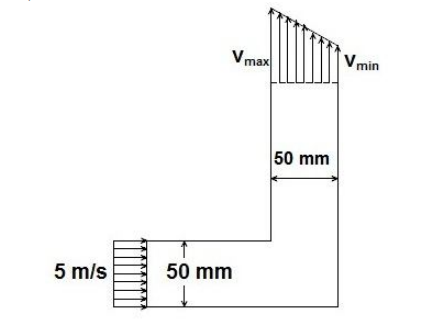
\includegraphics[width=0.5\columnwidth]{figs/fig4.png}
    \caption{}
    \label{fig:fig4}
\end{figure}
\begin{multicols}{4}
\begin{enumerate}
\item 25
\item 2.5
\item 2.0
\item 0.2
\end{enumerate}
\end{multicols}

\item The velocity vector corresponding to a flow field is given by $\vec{V} = 3x \hat{i} + 4 y \hat{j}$. The magnitude of rotation at the point (2,2) in rad/s is: \hfill[GATE 2013 XE]

\begin{multicols}{4}
\begin{enumerate}
\item 0.75
\item 1.33
\item 2
\item 4
\end{enumerate}
\end{multicols}

\item The stream function for a potential flow field is given by $\psi = x^2 - y^2$. The corresponding potential function, assuming zero potential at the origin, is: \hfill[GATE 2013 XE]

\begin{multicols}{4}
\begin{enumerate}
\item $x^2 + y^2$
\item $2xy$
\item $x^2 - y^2$
\item $x - y$
\end{enumerate}
\end{multicols}

\item Fully developed flow of an oil takes place in a pipe of inner diameter 50 mm. The pressure drop per metre length of the pipe is 2 kPa. Determine the shear stress, in Pa, at the pipe wall  \underline{\hspace{1.5cm}}.\hfill[GATE 2013 XE]

\item The Darcy friction factor $f$ for a smooth pipe is given by $f=64/\text{Re}$ for laminar flow and by $f=0.3/\text{Re}^{0.25}$ for turbulent flow, where Re is the Reynolds number based on the diameter. For fully developed flow of a fluid of density 1000 kg/m$^3$ and dynamic viscosity 0.001 Pa.s through a smooth pipe of diameter 10 mm with a velocity of 1 m/s, determine the Darcy friction factor \underline{\hspace{1.5cm}}. \hfill[GATE 2013 XE]



\item Air flows steadily through a channel. The stagnation and static pressures at a point in the flow are measured by a Pitot tube and a wall pressure tap, respectively. The pressure difference is found to be 20 mm Hg. The densities of air, water and mercury, in kg/m$^3$, are 1.18, 1000 and 13600, respectively. The gravitational acceleration is 9.81 m/s$^2$. Determine the air speed in m/s \underline{\hspace{1.5cm}}. \hfill[GATE 2013 XE]

\subsection{common data 38 and 39} 
The velocity field within a laminar boundary layer is given by the expression:
 \begin{align}
\vec{V} = \frac{Bu_{\infty}y}{x^{3/2}}\hat{i} + \frac{Bu_{\infty}y^2}{4x^{5/2}}\hat{j}
\end{align}
where $u = 100 y^{1/2}$ m/s and $v = 0.01 x / y$ m/s. The free stream velocity $U_{\infty} = 0.1$ m/s.
\item Calculate the x-direction component of the acceleration in m/s$^2$ at the point $x=0.5$ m and $y=50$mm\underline{\hspace{1.5cm}}. \hfill[GATE 2013 XE]

\item Find the slope of the streamline passing through the point $x=0.5$ m and $y=50$ mm\underline{\hspace{1.5cm}}. \hfill[GATE 2013 XE]

\subsection{common data for 40 and 41}
The wave and eddy resistance of a sea-going vessel, 96 m in length, driven at a velocity of 12 m/s, is to be determined. For this purpose, a 1/16$^\text{th}$ scale model is employed in fresh water and the coefficient of resistance $C_{we}$ of the model is found to be $1.47 \times 10^{-4}$. The quantity $C_{we}$ is defined as $C_{we} = R_{we} / brak{\frac{1}{2} \rho V^2 L}$, where $R_{we}$ is the wave and eddy resistance, $\rho$ is the fluid density, $V$ is the velocity and $L$ is the characteristic length. The density of sea water is 1026 kg/m$^3$.
\item The velocity in m/s, at which the model is towed, is: \hfill[GATE 2013 XE]

\begin{multicols}{4}
\begin{enumerate}
\item 0.75
\item 1.33
\item 3
\item 192
\end{enumerate}
\end{multicols}

\item The resistance of the prototype, in kN, is: \hfill[GATE 2013 XE]

\begin{multicols}{4}
\begin{enumerate}
\item 6
\item 25
\item 26.9
\item 100.1
\end{enumerate}
\end{multicols}
\subsection{common data for 42 and 43}
 Water enters a symmetric forked pipe and discharges into atmosphere through the two branches as shown in the figure. The cross-sectional area of section-1 is 0.2 m$^2$ and the velocity across section-1 is 3 m/s. The density of water may be taken as 1000 kg/m$^3$. The viscous effects and elevation changes may be neglected. 
 \begin{figure}[H]
     \centering
     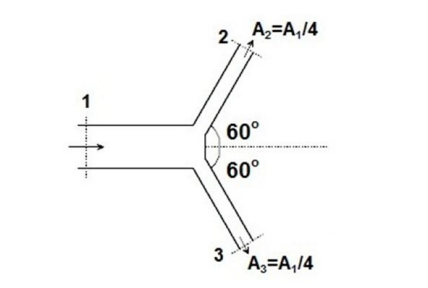
\includegraphics[width=0.5\columnwidth]{figs/fig5.png}
     \caption{}
     \label{fig:fig6}
 \end{figure}
\item The gauge pressure at section-1, in kPa, is: \hfill[GATE 2013 XE]

\begin{multicols}{4}
\begin{enumerate}
\item 0.6
\item 13.5
\item 135
\item 600
\end{enumerate}
\end{multicols}

\item The magnitude of the force, in kN, required to hold the pipe in place, is: \hfill[GATE 2013 XE]

\begin{multicols}{4}
\begin{enumerate}
\item 2.7
\item 5.4
\item 19
\item 27
\end{enumerate}
\end{multicols}

\begin{center}
\begin{tabular}[12pt]{|l|l|}
\hline 
  P.Processes   & 1.Characteristics / Applications \\ \hline
  Q.Gas Metal Arc Welding    & 2.Joining of thick plates \\ \hline
  R.Tungsten Inert Gas Welding &  3.Consumable electrode wire  \\ \hline
  S.Electroslag Welding & 4.Joining of cylindrical dissimilar materials \\ \hline
\end{tabular}
\end{center}

\item As temperature increases, diffusivity of an atom in a solid material,\hfill[GATE 2013 XE]
\begin{multicols}{2}
\begin{enumerate}
\item increases
\item decreases
\item remains constant
\item depends on the specific material
\end{enumerate}
\end{multicols}

\item Which of the following is NOT correct?\hfill[GATE 2013 XE]
\begin{multicols}{2}
\begin{enumerate}
\item Dislocations are thermodynamically unstable defects.
\item Dislocations can move inside a crystal under the action of an applied stress.
\item Screw dislocations can change the slip plane without climb.
\item Burger's vector of an edge dislocation is parallel to the dislocation line.
\end{enumerate}
\end{multicols}

\item At a constant atmospheric pressure, the number of phases, $P$, which coexist in a system at equilibrium, is related to the number of components, $C$, and degree of freedom, $F$ by\hfill[GATE 2013 XE]
\begin{multicols}{2}
\begin{enumerate}
\item $P+F=C-2$
\item $P+F=C+2$
\item $P+F=C+1$
\item $P+F=C-1$
\end{enumerate}
\end{multicols}

\item Which one of the following metals is commonly alloyed with iron to improve its corrosion resistance?\hfill[GATE 2013 XE]
\begin{multicols}{2}
\begin{enumerate}
\item Co
\item Cr
\item Ti
\item Nb
\end{enumerate}
\end{multicols}

\item The number of slip systems in a metal with FCC crystal structure is\hfill[GATE 2013 XE]
\begin{multicols}{2}
\begin{enumerate}
\item 4
\item 6
\item 8
\item 12
\end{enumerate}
\end{multicols}

\item Upon recrystallization of a cold worked metal,\hfill[GATE 2013 XE]
\begin{multicols}{2}
\begin{enumerate}
\item strength increases and ductility decreases
\item strength decreases but ductility increases
\item both strength and ductility increase
\item both strength and ductility decrease
\end{enumerate}
\end{multicols}

\item  In carbon fiber reinforced resin composites, for a given fiber volume content, Young’s modulus depends on fiber orientation with respect to load. Maximum value occurs when\hfill[GATE 2013 XE]
\begin{multicols}{2}
\begin{enumerate}
\item transverse
\item longitudinal
\item random
\item both transverse and longitudinal
\end{enumerate}
\end{multicols}

\item Vulcanization is related to\hfill[GATE 2013 XE]
\begin{multicols}{2}
\begin{enumerate}
\item strengthening of rubber
\item extrusion
\item injection moulding
\item addition polymerisation
\end{enumerate}
\end{multicols}

\item Which one of the following oxides crystallizes into fluorite structure?\hfill[GATE 2013 XE]
\begin{multicols}{2}
\begin{enumerate}
\item UO$_2$
\item MgO
\item BaTiO$_3$
\item MgAl$_2$O$_4$
\end{enumerate}
\end{multicols}
\item Match the conventional ceramic materials listed in Column I with their respective common applications in Column II\hfill[GATE 2013 XE]

\begin{tabular}{ll}
\textbf{Column I} & \textbf{Column II} \\
P. Lead Zirconate Titanate (PZT) & 1. cutting tool \\
Q. Zinc Oxide (ZnO) & 2. thermal barrier coating \\
R. Silicon Carbide (SiC) & 3. actuator \\
S. Zirconia (ZrO$_2$) & 4. varistor \\
& 5. super conductor \\
\end{tabular}

\begin{enumerate}
\item P-1, Q-2, R-3, S-5
\item P-3, Q-2, R-1, S-5
\item P-2, Q-1, R-5, S-3
\item P-3, Q-4, R-1, S-2
\end{enumerate}



\item Match the terminologies given in Column I with their relations listed in Column II\hfill[GATE 2013 XE]

\begin{tabular}{ll}
\textbf{Column I} & \textbf{Column II} \\
P. domain wall & 1. superconductors \\
Q. Fick's law & 2. mechanical properties \\
R. Matthiessen's rule & 3. ferromagnetic materials \\
S. Hall-Petch relation & 4. resistivity of impure metals \\
T. Meissner effect & 5. diffusion \\
\end{tabular}

\begin{enumerate}
\item P-1, Q-3, R-5, S-2, T-4
\item P-3, Q-5, R-2, S-4, T-1
\item P-3, Q-5, R-4, S-2, T-1
\item P-3, Q-4, R-3, S-2, T-4
\end{enumerate}



\item Match the microscopes listed in Column I with their principle of operation listed in Column II\hfill[GATE 2013 XE]

\begin{tabular}{ll}
\textbf{Column I} & \textbf{Column II} \\
P. Scanning Electron Microscope (SEM) & 1. van der Waals forces between atoms \\
Q. Transmission Electron Microscope (TEM) & 2. electrons to jump across a potential barrier \\
R. Scanning Tunnelling Microscope (STM) & 3. diffraction of electrons \\
S. Atomic Force Microscope (AFM) & 4. detection of secondary electrons \\
& 5. photo emission of electrons \\
\end{tabular}

\begin{enumerate}
\item P-2, Q-5, R-3, S-1
\item P-3, Q-4, R-5, S-2
\item P-4, Q-3, R-2, S-1
\item P-4, Q-3, R-5, S-2
\end{enumerate}
\item X-rays of unknown wavelength are diffracted by an FCC metal with a lattice parameter of $0.352\ \mathrm{nm}$. The measured $2\theta$ angle for the $\{200\}$ peak is $61.08^\degree$. Calculate the wavelength of the X-ray used, in nm. \underline{\hspace{2cm}}\hfill[GATE 2013 XE]

\item A metal with HCP crystal structure has lattice constants $a = 0.30\ \mathrm{nm}$ and $c = 0.56\ \mathrm{nm}$. Determine the volume of the unit cell of this metal, in $\mathrm{nm}^3$. \underline{\hspace{2cm}}\hfill[GATE 2013 XE]

\item The band gap of a semiconducting material used to make an LED is $1.43\ \mathrm{eV}$. What will be the minimum wavelength of the radiation emitted by this LED, in $\mu\mathrm{m}$? \underline{\hspace{2cm}}\hfill[GATE 2013 XE]

\item For automatic control of household electric water heater, a relay switch is activated by thermal expansion of a brass rod of length $50\ \mathrm{cm}$ as shown in the schematic below. 
The distance between the rod and the lever, $x$, is adjusted by moving the base of the rod. As the water gets heated, the rod expands and as soon as the rod touches the lever, the circuit is broken disconnecting the heater from the power supply. Find the distance, $x$, in mm, to be set at water temperature of $20^\degree$C such that the circuit is broken at $70^\degree$C. The coefficient of linear thermal expansion of brass is $20 \times 10^{-6}\ ^\degree\mathrm{C}^{-1}$. \underline{\hspace{2.5cm}}.
\begin{figure}[H]
    \centering
    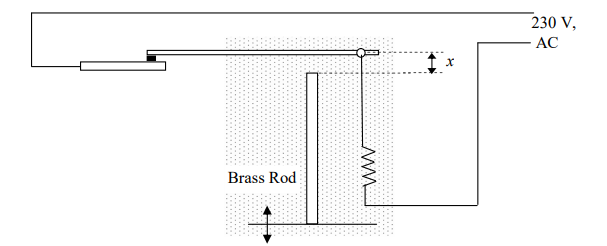
\includegraphics[width=0.5\columnwidth]{figs/fig6.png}
    \caption{}
    \label{fig:fig6}
\end{figure}
\textbf{Common Data for Questions 60 and 61:}  

From tensile test of a particular alloy, the following values were obtained.  
The material exhibits linear work hardening as shown in the figure below.
% Placeholder for stress-strain figure


\begin{tabular}{|c|c|c|}
\hline
 & \textbf{At Yield} & \textbf{At Fracture} \\
\hline
Stress (GPa) & 0.7 & 0.8 \\
Strain (\%) & 1 & 4 \\
\hline
\end{tabular}
\begin{figure}[H]
    \centering
    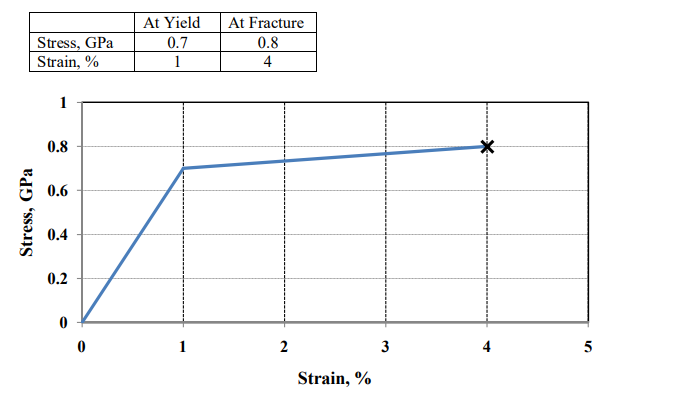
\includegraphics[width=0.5\columnwidth]{figs/fig7.png}
    \caption{}
    \label{fig:fig7}
\end{figure}
\item If the cylindrical specimen had a diameter of $10\ \mathrm{mm}$ and a length of $50\ \mathrm{mm}$, find the length of the specimen at the yield point, in mm. \underline{\hspace{2cm}} \hfill[GATE 2013 XE]

\item Find the toughness of the material, in $\mathrm{MJ\ m^{-3}}$. \underline{\hspace{2cm}} \hfill[GATE 2013 XE]

\textbf{Common Data for Questions 63 and 62:}  

An isomorphous alloy system contains $47 \ \mathrm{wt\%}$ of A and $53 \ \mathrm{wt\%}$ of B and is at $1300^\degree$C.  
Referring to the phase diagram shown below, answer the following:
% Placeholder for phase diagram image
\begin{figure}[H]
    \centering
    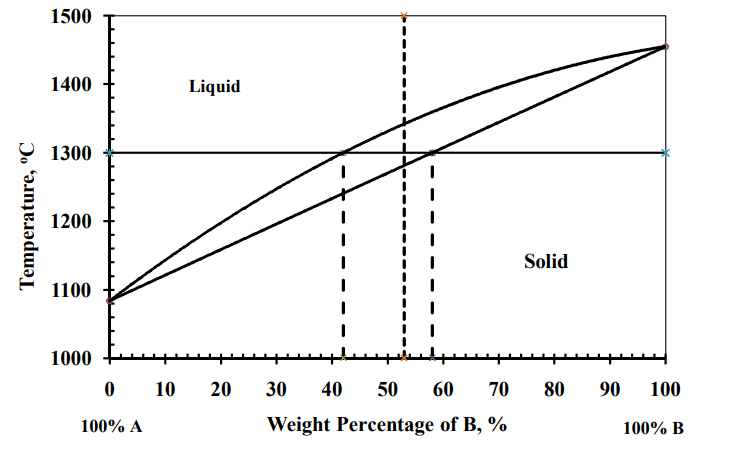
\includegraphics[width=0.5\columnwidth]{figs/fig8.png}
    \caption{}
    \label{fig:fig 8}
\end{figure}
\item What is the weight percentage of A in solid phase at this temperature? \underline{\hspace{2cm}} \hfill[GATE 2013 XE]

\item What weight percentage of this alloy is liquid? \underline{\hspace{2cm}}\hfill[GATE 2013 XE]

\textbf{Linked Answer Questions — Statement for Q.64 and Q.65:}  

A stress of $10\ \mathrm{MPa}$ is applied to an elastomer to generate a strain of 50\%. The strain is held constant at this value. After 40 days at $20^\degree$C, the stress decreases to $5\ \mathrm{MPa}$.

\item What is the \textbf{relaxation time constant} for this material? \underline{\hspace{2cm}}\hfill[GATE 2013 XE]

\item What will be the \textbf{stress after 60 days} at $20^\degree$C? \underline{\hspace{2cm}}\hfill[GATE 2013 XE]

\item At a point in a body subjected to plane stress, the state of stress is as shown in the Figure. One of the principal stresses is $180 \ \mathrm{MPa}$. Find the unknown shear stress $\tau$ (in MPa). \underline{\hspace{2cm}}\hfill[GATE 2013 XE]

\begin{figure}[H]
    \centering
    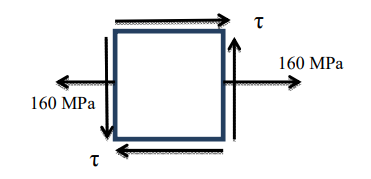
\includegraphics[width=0.5\columnwidth]{figs/fig9.png}
    \caption{}
    \label{fig:fig9}
\end{figure}

\item A point in a body is subjected to a hydrostatic pressure of $100 \ \mathrm{MPa}$. Find the maximum shear stress at this point in MPa. \underline{\hspace{2cm}}\hfill[GATE 2013 XE]

\item A circular shaft of diameter $10 \ \mathrm{mm}$ and length $3 \ \mathrm{m}$ is subjected to a torque of $T=\pi \ \mathrm{N\cdot m}$ at a location $2 \ \mathrm{m}$ away from the fixed end as shown in the Figure. Find the angle of twist (in radians) at the free end. Shear modulus of the material of the shaft is $10 \ \mathrm{GPa}$. \underline{\hspace{2cm}}\hfill[GATE 2013 XE]
\begin{figure}[H]
    \centering
    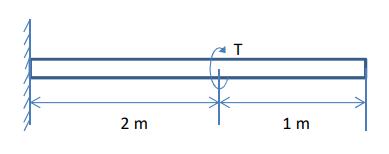
\includegraphics[width=0.5\columnwidth]{figs/fig10.png}
    \caption{}
    \label{fig:fig10}
\end{figure}

\item A rigid massless rod ABC is hinged at A and carries a point mass $M$ (in kg) at C. Point B is connected to a linear spring with spring constant $k$ (in N/m) as shown in the figure. The length AB and AC are $a$ and $L$, respectively. Neglecting the effect of gravity, the natural frequency of this spring–mass system in rad/s is:\hfill[GATE 2013 XE]

\begin{figure}[H]
    \centering
    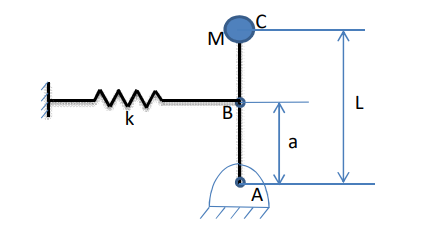
\includegraphics[width=0.5\columnwidth]{figs/fig11.png}
    \caption{}
    \label{fig:fig11}
\end{figure}

\begin{multicols}{4}
\begin{enumerate}
\item $\sqrt{\frac{k L^2}{Ma^2}}$
\item $\sqrt{\frac{ka}{Ml}}$
\item $\sqrt{\frac{ka^2}{ML^2}}$
\item $\sqrt{\frac{kL}{Ma}}$
\end{enumerate}
\end{multicols}

\item A two–bar truss is shown in the Figure. The cross–sectional area and Young’s modulus of bar 1 are $0.02 \ \mathrm{m^2}$ and $200 \ \mathrm{GPa}$, respectively. The cross–sectional area and Young’s modulus of bar 2 are $0.01 \ \mathrm{m^2}$ and $80 \ \mathrm{GPa}$, respectively. The force $F$ applied on the truss is $2 \ \mathrm{N}$. Find the stress developed in bar 2 in Pa. \underline{\hspace{2cm}}
\begin{figure}[H]
    \centering
    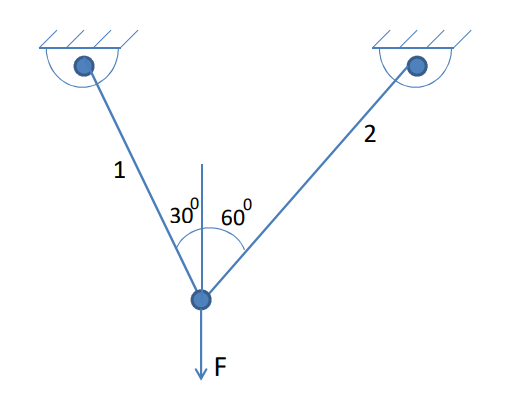
\includegraphics[width=0.5\columnwidth]{figs/fig12.png}
    \caption{}
    \label{fig:fig12}
\end{figure}
\item A spring balance reads $10 \ \mathrm{kg}$ in a lift when the lift is stationary. When the lift starts moving with a constant acceleration, the new reading is $12.3 \ \mathrm{kg}$. If the upward acceleration is considered positive, what is the acceleration of the lift? Acceleration due to gravity may be taken as $10 \ \mathrm{m/s^2}$ downwards. \underline{\hspace{2cm}}

\item A force $F=2 \ \mathrm{N}$ is applied on a block of mass $M=0.5 \ \mathrm{kg}$ as shown in the figure. The block is constrained to move along the horizontal direction in a guideway. Find the distance (in meters) travelled by the block in $2 \ \mathrm{s}$ starting from rest. Neglect any friction between the block and the guideway. \underline{\hspace{2cm}}
\begin{figure}[H]
    \centering
    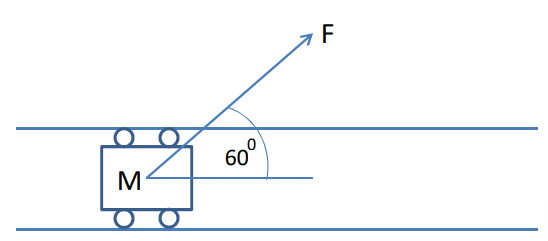
\includegraphics[width=0.5\columnwidth]{figs/fig13.png}
    \caption{}
    \label{fig:fig13}
\end{figure}
\item A man of mass $50 \ \mathrm{kg}$ is walking on a long wooden board of mass $200 \ \mathrm{kg}$ (as shown in the Figure). The wooden board is initially at rest on a frictionless ice surface. If the man walks with a velocity $V=1 \ \mathrm{m/s}$ in the positive $x$ direction relative to the wooden board, find the velocity of the board in m/s. Velocity is positive in the positive $x$ direction. \underline{\hspace{2cm}}
\begin{figure}[H]
    \centering
    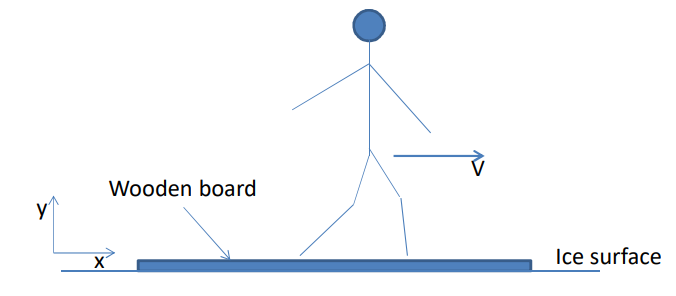
\includegraphics[width=0.5\columnwidth]{figs/fig14.png}
    \caption{}
    \label{fig:fig14}
\end{figure}
\item A rigid bar AB is hinged at B through a torsional spring with spring constant $k_t$. For small rotations of the bar AB about B, the critical load $P_{cr}$ is given by:

\begin{figure}[H]
    \centering
    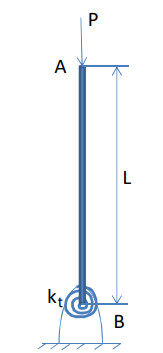
\includegraphics[width=0.5\columnwidth]{figs/fig15.png}
    \caption{}
    \label{fig:fig15}
\end{figure}

\begin{multicols}{2}
\begin{enumerate}
\item $\frac{\pi^2 E I}{L^2}$
\item $\frac{\pi^2 E I}{L}$
\item $\frac{E I}{L^3}$
\item $\frac{k_t}{L}$
\end{enumerate}
\end{multicols}

\item A disk of mass $M=14 \ \mathrm{kg}$ and radius $1 \ \mathrm{m}$ is attached to a spring which has a stiffness $k=75 \ \mathrm{N/m}$ and an unstretched length of $1 \ \mathrm{m}$. If the disk is released from rest in the position shown in the Figure and the disk rolls without slipping, find its angular velocity (in rad/s) at the instant the center of mass is displaced by $3 \ \mathrm{m}$. \underline{\hspace{2cm}}

\begin{figure}[H]
    \centering
    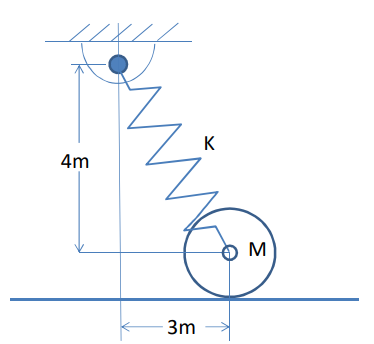
\includegraphics[width=0.5\columnwidth]{figs/fig16.png}
    \caption{}
    \label{fig:fig16}
\end{figure}

\item A strain gauge is mounted on the outer surface of a thin cylindrical pressure vessel in the circumferential direction. The mean diameter and thickness of the cylinder are $4.0 \ \mathrm{m}$ and $20 \ \mathrm{mm}$, respectively. Young’s modulus and Poisson’s ratio of the material of the cylinder are $200 \ \mathrm{GPa}$ and $0.25$, respectively. Find the pressure in MPa inside the cylindrical vessel when the strain gauge indicates a strain of $7.0\times 10^{-4}$. \underline{\hspace{2cm}}

\item A solid shaft of diameter $100 \ \mathrm{mm}$ is rotating at a constant angular speed of $(10/\pi) \ \mathrm{rad/s}$. The shaft carries three rigid pulleys A, B and C as shown in the Figure. Pulley B is connected to a motor supplying $10\ \mathrm{kW}$ power. Pulley B and C are connected to two pumps consuming $5\ \mathrm{kW}$ each. Find the maximum shear stress (in MPa) in the shaft due to torsion alone. \underline{\hspace{2cm}}

\begin{figure}[H]
    \centering
    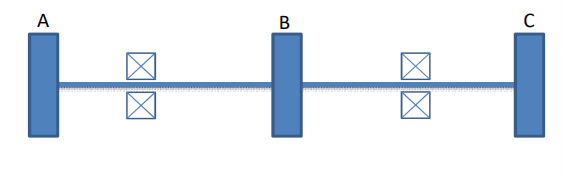
\includegraphics[width=0.5\columnwidth]{figs/fig17.png}
    \caption{}
    \label{fig:fig17}
\end{figure}

\item A beam is fixed at the left end and supported by a spring at the other end. The length of the beam is $L$ and its flexural rigidity is $EI$. The spring constant of the spring is $k=\frac{3EI}{L^3}$. A vertical downward load $P$ is applied at the right end. The deflection of the point under the load $P$ is:

\begin{figure}[H]
    \centering
    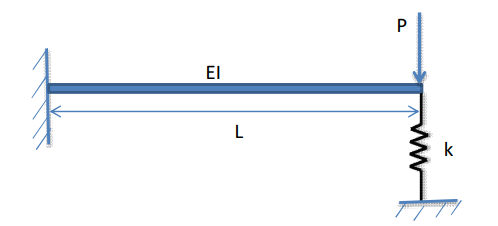
\includegraphics[width=0.5\columnwidth]{figs/fig18.png}
    \caption{}
    \label{fig:fig18}
\end{figure}

\begin{multicols}{2}
\begin{enumerate}
\item $\frac{P L^3}{9EI}$
\item $\frac{P L^3}{6EI}$
\item $\frac{2P L^3}{9EI}$
\item $\frac{5P L^3}{9EI}$
\end{enumerate}
\end{multicols}

\item Find the maximum bending moment (magnitude wise) in kN–m for the beam shown in the Figure. \underline{\hspace{2cm}}

\begin{figure}[H]
    \centering
    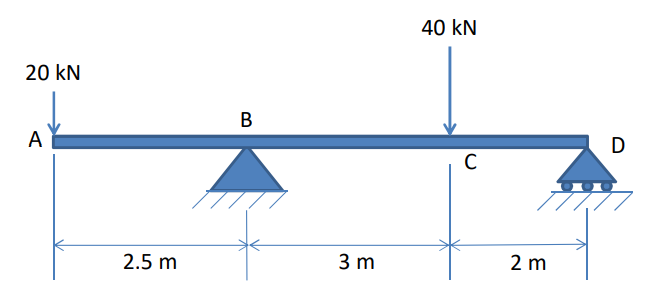
\includegraphics[width=0.5\columnwidth]{figs/fig19.png}
    \caption{}
    \label{fig:fig19}
\end{figure}

\item A projectile is fired with velocity $V=3\sqrt{2} \ \mathrm{m/s}$ from a point at height $H=0.8 \ \mathrm{m}$ at an angle of $45^\degree$ with respect to the horizontal directionn as shown in the Figure. Find the horizontal distance S in
meters travelled by the projectile when it hits the ground. Take $g=10 \ \mathrm{m/s^2}$. Find the horizontal distance $S$ in meters travelled when it hits the ground. \underline{\hspace{2cm}}

\begin{figure}[H]
    \centering
    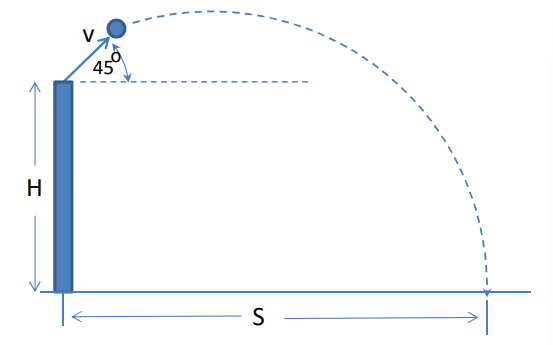
\includegraphics[width=0.5\columnwidth]{figs/fig20.png}
    \caption{}
    \label{fig:fig20}
\end{figure}

\item A  particle P is moving on a circular path of radius $r=1\ \mathrm{m}$ . The angular location  of the particle is
measured as shown in the Figure. The motion of the particle is described by $\theta(t)= 2\sin t$. Find the
magnitude of the total acceleration (in m/s2
) of the particle at time  $t=\pi/3$ s (m/s$^2$): \underline{\hspace{2cm}}

\begin{figure}[H]
    \centering
    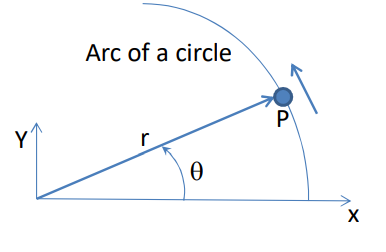
\includegraphics[width=0.5\columnwidth]{figs/fig21.png}
    \caption{}
    \label{fig:fig21}
\end{figure}

 \textbf{Common Data for Q.17–Q.18:} A frame ABC is shown in the Figure. Members AB and BC both have length $L$ and Young’s modulus $E$. Members AB and BC both have a square cross-section of side a. A load P is applied at point C as
shown in the figure.

\begin{figure}[H]
    \centering
    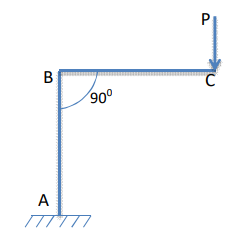
\includegraphics[width=0.5\columnwidth]{figs/fig22.png}
    \caption{}
    \label{fig:fig22}
\end{figure}

\item Neglecting axial compression of AB, the deflection of C in the direction of the load is:

\begin{multicols}{2}
\begin{enumerate}
\item $\frac{P L^3}{3EI}$
\item $\frac{P L^3}{6EI}$
\item $\frac{P L^3}{8EI}$
\item $\frac{P L^3}{12EI}$
\end{enumerate}
\end{multicols}

\item The maximum bending stress in the frame is:

\begin{multicols}{2}
\begin{enumerate}
\item $\frac{P L}{a^3}$
\item $\frac{2P L}{a^3}$
\item $\frac{3P L}{a^3}$
\item $\frac{4P L}{a^3}$
\end{enumerate}
\end{multicols}



 \textbf{Common Data for Q.19–Q.20:} Plane stress state shown.

\begin{figure}[H]
    \centering
    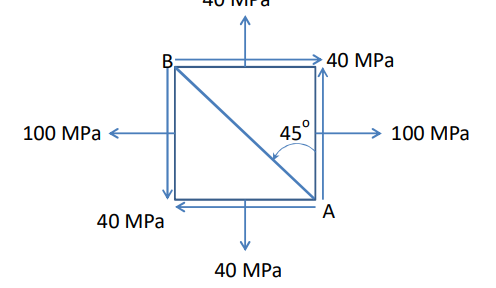
\includegraphics[width=0.5\columnwidth]{figs/fig23.png}
    \caption{}
    \label{fig:fig23}
\end{figure}
 
 \item One principal stress (MPa):\hfill[GATE 2013 XE]  
\begin{multicols}{4}
\begin{enumerate}
\item 40
\item 80
\item 120
\item 140
\end{enumerate}
\end{multicols}

\item Normal stress on plane AB (MPa):\hfill[GATE 2013 XE]  
\begin{multicols}{4}
\begin{enumerate}
\item 30
\item 70
\item 100
\item 110
\end{enumerate}
\end{multicols}

 \textbf{Linked Answer Q.21–Q.22:} 
 Two rods are joined together and the entire assembly is supported between two rigid walls, as shown in the
Figure. The cross-sectional area and Young’s modulus for both the rods are  $A=0.01\ \mathrm{m^2}$
and $10\ \mathrm{GPa}$, respectively.
The coefficients of thermal expansion for the two rods are $\alpha_1=4\times 10^{-6}/^\degree\mathrm{C}$, $\alpha_2=10^{-6}/^\degree\mathrm{C}$, respectively. The
entire assembly is heated by $100^\degree\mathrm{C}$. Neglect the effect of Poisson’s ratio.

\begin{figure}[H]
    \centering
    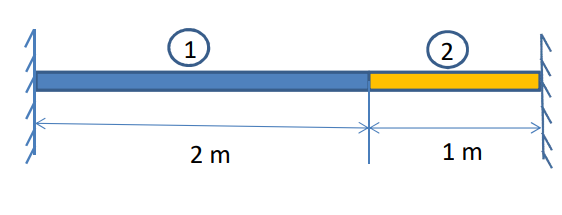
\includegraphics[width=0.5\columnwidth]{figs/fig24.png}
    \caption{}
    \label{fig:fig24}
\end{figure}
  
\item Stress in rod 1 (MPa):\hfill[GATE 2013 XE]  
\begin{multicols}{4}
\begin{enumerate}
\item $-4.0$
\item $-3.0$
\item $-2.5$
\item $-1.0$
\end{enumerate}
\end{multicols}

\item Considering the displacement to the right as positive, the displacement (in mm) of the interface
between the two rods is:\hfill[GATE 2013 XE]  
\begin{multicols}{4}
\begin{enumerate}
\item $-0.4$
\item $-0.1$
\item $0.1$
\item $0.4$
\end{enumerate}
\end{multicols}


\item The measured temperature of a system is $30^\degree$C. Its exact absolute temperature in K is \hfill[GATE 2013 XE]
\begin{multicols}{4}
\begin{enumerate}
\item 303.00
\item 303.10
\item 303.15
\item 303.16
\end{enumerate}
\end{multicols}

\item The fuel air mixture in a petrol engine is ignited with a spark plug at the end of compression stroke. This process \hfill[GATE 2013 XE]
\begin{multicols}{2}
\begin{enumerate}
\item increases the entropy of the fuel air mixture but decreases the entropy of the spark plug
\item decreases the entropy of the fuel air mixture but increases the entropy of the spark plug
\item decreases the entropy of the fuel air mixture and of the spark plug
\item increases the entropy of the fuel air mixture and of the spark plug
\end{enumerate}
\end{multicols}

\item In the van der Waals equation of state given below: \hfill[GATE 2013 XE]
\begin{align}
    \brak{p + \frac{a}{v^2}}\brak{v - b} = RT
\end{align}

The constant $a$ represents the effect of
\begin{multicols}{2}
\begin{enumerate}
\item attractive forces between molecules
\item repulsive forces between molecules
\item deviation from molecules being spherical
\item finite size of the molecule
\end{enumerate}
\end{multicols}

\item For a reversible isothermal expansion of an ideal gas from a state 1 to a state 2, \hfill[GATE 2013 XE]
\begin{multicols}{4}
\begin{enumerate}
\item $s_1 = s_2$
\item $s_1 > s_2$
\item $s_1 < s_2$
\item $h_1 > h_2$
\end{enumerate}
\end{multicols}

\item For a pure substance the critical isotherm on the $p-v$ plane exhibits \hfill[GATE 2013 XE]
\begin{multicols}{4}
\begin{enumerate}
\item a maximum
\item a minimum
\item a point of inflection
\item a discontinuity
\end{enumerate}
\end{multicols}

\item For an ideal gas as a working fluid for a given heat input $Q$, the process that gives the maximum work among the following four processes is \hfill[GATE 2013 XE]
\begin{multicols}{4}
\begin{enumerate}
\item isothermal
\item constant volume
\item constant pressure
\item isentropic
\end{enumerate}
\end{multicols}

\item An air standard Otto cycle has the following shape on a thermodynamic property plane. \hfill[GATE 2013 XE]

\begin{figure}[H]
    \centering
    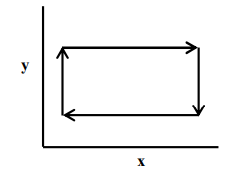
\includegraphics[width=0.5\columnwidth]{figs/fig25.png}
    \caption{}
    \label{fig:fig25}
\end{figure}
The $x$ and $y$ coordinates, respectively, are
\begin{multicols}{4}
\begin{enumerate}
\item $v$ and $p$
\item $s$ and $v$
\item $v$ and $T$
\item $s$ and $p$
\end{enumerate}
\end{multicols}

\item The specific volume of steam after expansion in a turbine is $12 \ \mathrm{m^3/kg}$. At this pressure the saturated liquid and saturated vapour specific volumes are $0.001$ and $15.25 \ \mathrm{m^3/kg}$ respectively. What is the dryness fraction to second decimal place accuracy? \underline{\hspace{2cm}} \hfill[GATE 2013 XE]

\item Which of the following processes, shown in the figure below, represents the throttling of an ideal gas? \hfill[GATE 2013 XE]

\begin{figure}[H]
    \centering
    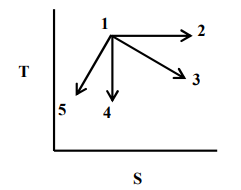
\includegraphics[width=0.5\columnwidth]{figs/fig26.png}
    \caption{}
    \label{fig:fig26}
\end{figure}

\begin{multicols}{4}
\begin{enumerate}
\item 1 to 2
\item 1 to 3
\item 1 to 4
\item 1 to 5
\end{enumerate}
\end{multicols}

\item On a $\ln p$ vs $h$ coordinate system, where $\ln p$ is the $y$-coordinate and $h$ is the $x$ coordinate, the slope of a constant entropy line is \hfill[GATE 2013 XE]
\begin{multicols}{4}
\begin{enumerate}
\item $1/v$
\item $v$
\item $p/v$
\item $1/(pv)$
\end{enumerate}
\end{multicols}


\item Starting from the definition of Gibbs free energy function $g = h - Ts$, the Maxwell relation that can be derived is \hfill[GATE 2013 XE]
\begin{multicols}{4}
\begin{enumerate}
\item $\brak{ \frac{\partial T}{\partial p} }_{s} = \brak{ \frac{\partial v}{\partial s} }_{p}$
\item $\brak{ \frac{\partial T}{\partial p} }_{s} = v$
\item $\brak{ \frac{\partial s}{\partial p} }_{T} = - \brak{ \frac{\partial v}{\partial T} }_{p}$
\item $\brak{ \frac{\partial s}{\partial p} }_{T} = - \brak{ \frac{\partial p}{\partial T} }_{v}$
\end{enumerate}
\end{multicols}
\item A thermodynamic cycle operates between one source at a temperature of $600\ \mathrm{K}$, another source at a temperature of $300\ \mathrm{K}$ and a sink at a temperature $T$ as shown in the figure below. If the First and Second laws of thermodynamics are not violated, what should be the value of $T$ in K? \underline{\hspace{2cm}}

\hfill[GATE 2013 XE]

\begin{figure}[H]
    \centering
    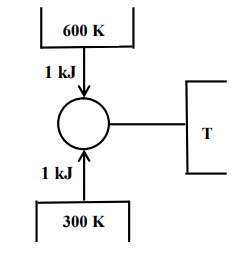
\includegraphics[width=0.5\columnwidth]{figs/fig27.png}
    \caption{}
    \label{fig:fig 27}
\end{figure}

\item A closed system containing an ideal gas undergoes a cycle as shown in the figure below. For the process 1–2, which one of the following statements is true?

\hfill[GATE 2013 XE]

\begin{figure}[H]
    \centering
    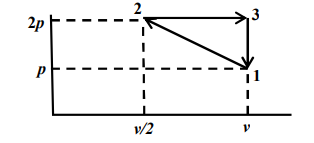
\includegraphics[width=0.5\columnwidth]{figs/fig28.png}
    \caption{}
    \label{fig:fig28}
\end{figure}

\begin{multicols}{2}
\begin{enumerate}
\item Heat added $= p v \ln 2$
\item Heat rejected $= p v \ln 2$
\item Heat added $= p v$
\item Heat rejected $= p v$
\end{enumerate}
\end{multicols}

\item A well-insulated rigid hot water tank receives steady flow of water from two sources as shown in the figure below. There is no accumulation of water in the tank. A back-up heater is provided to ensure a constant outflow temperature of water at $60^\degree\mathrm{C}$ from the tank under steady state. What is the required capacity of the back-up heater to the nearest kW? \underline{\hspace{2cm}}

\hfill[GATE 2013 XE]

\begin{figure}[H]
    \centering
    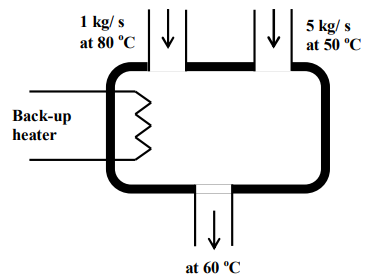
\includegraphics[width=0.5\columnwidth]{figs/fig29.png}
    \caption{}
    \label{fig:fig29}
\end{figure}

\item $1\ \mathrm{kg}$ of air in an insulated rigid tank of volume $1\ \mathrm{m^3}$ is churned with a frictionless fan of $600\ \mathrm{W}$ capacity for $10$ minutes. The fan efficiency is 100\%. Treating air as an ideal gas and neglecting kinetic and potential energy changes, what is the increase of pressure, to the nearest kPa? \underline{\hspace{2cm}}

\hfill[GATE 2013 XE]

\begin{figure}{H}
    \centering
    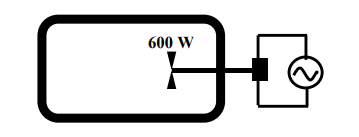
\includegraphics[width=0.5\columnwidth]{figs/fig30.png}
    \caption{}
    \label{fig:fig30}
\end{figure}

\item The isothermal compressibility of a liquid is $5\times 10^{-6}\ \mathrm{/kPa}$. If it is compressed at constant temperature from $5000$ to $10000\ \mathrm{kPa}$, what is the ratio of final volume to initial volume, to second decimal place accuracy? \underline{\hspace{2cm}}

\hfill[GATE 2013 XE]

\textbf{common data for 104 and 105}

At a location where the atmospheric pressure is $98\ \mathrm{kPa}$ and the ambient temperature is $30^\degree\mathrm{C}$, the humidity ratio is $0.01\ \mathrm{kg/kg}$ of dry air. A high pressure front moves over the location which changes only the atmospheric pressure to $102\ \mathrm{kPa}$, while the humidity ratio remains the same. 
\item What is the partial pressure of water vapour in kPa to the first decimal place accuracy before the high pressure front moves in? \underline{\hspace{2cm}}

\hfill[GATE 2013 XE]

\item , what is the relative humidity of air under the influence of high pressure front to integer precision in \%? \underline{\hspace{2cm}}

\hfill[GATE 2013 XE]

\textbf{common data for 106 and 107}

 A rigid insulated cylinder is divided into two chambers A and B by a thin rigid insulating barrier as shown in the figure below. Initially, chamber A contains a mixture of $0.5\ \mathrm{kg}$ nitrogen and $0.5\ \mathrm{kg}$ helium at $300\ \mathrm{K}$ while chamber B contains $1\ \mathrm{kg}$ of pure nitrogen at $400\ \mathrm{K}$. The pressure in chamber B is twice that in chamber A. The gases and gas mixtures are assumed to be ideal.
 

\begin{figure}[H]
    \centering
    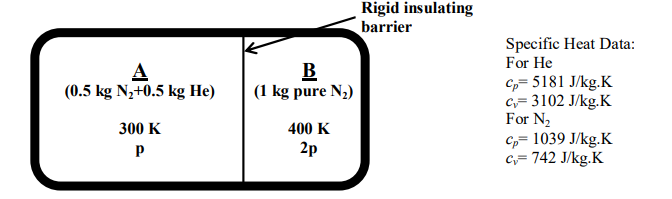
\includegraphics[width=0.5\columnwidth]{figs/fig31.png}
    \caption{}
    \label{fig:fig31}
\end{figure}

\item What is the ratio of the volumes of chambers A and B, i.e., $V_A / V_B$, to first decimal place accuracy? \underline{\hspace{2cm}}

\hfill[GATE 2013 XE]

\item For the same data as in Q.19, if the barrier is removed and the gases are allowed to mix and reach thermodynamic equilibrium, what is the final temperature of the mixture, to the nearest K? \underline{\hspace{2cm}}

\hfill[GATE 2013 XE]

\textbf{common data for 108 109 }

 A combined vapour compression-cum-Brayton cycle is shown below. 
 
\begin{figure}[H]
    \centering
    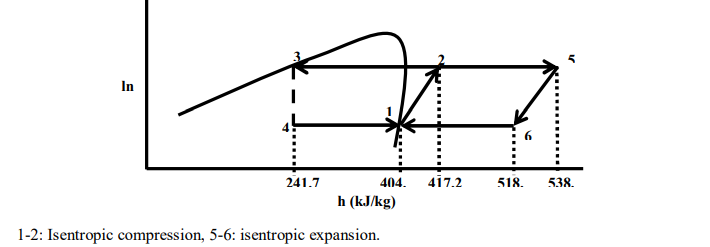
\includegraphics[width=0.5\columnwidth]{figs/fig32.png}
    \caption{}
    \label{fig:fig32}
\end{figure}

The refrigeration system has a cooling capacity of $30\ \mathrm{kW}$ and the turbine generates a power of $30\ \mathrm{kW}$.

\item What is the mass flow rate of the working fluid through the turbine, in kg/s, to first decimal place accuracy? \underline{\hspace{2cm}}

\hfill[GATE 2013 XE]



\item  what is the power required to drive the compressor, to the nearest kW? \underline{\hspace{2cm}}

\hfill[GATE 2013 XE]
  
\item In free radical polymerization, one of the following techniques permits simultaneous increase in rate of polymerization and polymer molecular weight. \hfill[GATE 2025 XE]

\begin{multicols}{2}
\begin{enumerate}
\item Solution polymerization
\item Suspension polymerization
\item Bulk polymerization
\item Emulsion polymerization
\end{enumerate}
\end{multicols}

\item The shear modulus, $G$, of plastic is related to the elastic modulus, $E$, and the Poisson ratio, $\nu$, as \hfill[GATE 2025 XE]

\begin{multicols}{2}
\begin{enumerate}
\item $E = 2(1-\nu)G$
\item $G = 2(1+\nu)E$
\item $E = 2(1+\nu)G$
\item $E = (1+\nu)G$
\end{enumerate}
\end{multicols}

\item LLDPE is obtained by \hfill[GATE 2025 XE]

\begin{multicols}{2}
\begin{enumerate}
\item Ziegler-Natta polymerization of ethylene
\item free-radical polymerization of ethylene
\item free-radical polymerization of ethylene and alpha-olefins
\item Ziegler-Natta copolymerization of ethylene and alpha-olefins
\end{enumerate}
\end{multicols}

\item A hindered phenol is added to a polyolefin \hfill[GATE 2025 XE]

\begin{multicols}{2}
\begin{enumerate}
\item to increase ozone resistance
\item to increase foamability
\item to increase oxidation resistance
\item to increase crosslinkability
\end{enumerate}
\end{multicols}

\item Stretching of rubber leads to \hfill[GATE 2025 XE]

\begin{multicols}{2}
\begin{enumerate}
\item decrease in alignment of polymer chains
\item increase in alignment of polymer chains
\item no change in alignment of polymer chains
\item decrease in strength of rubber
\end{enumerate}
\end{multicols}

\item In a cone and plate viscometer, the rate of strain is related to the speed of rotation of the cone, $\omega$ (radian/second), and the angle between the cone and the plate, $\alpha$ (radian), by the following relation \hfill[GATE 2025 XE]

\begin{multicols}{2}
\begin{enumerate}
\item $\omega \alpha$
\item $\omega \cos \alpha$
\item $\frac{\omega}{\alpha}$
\item $\frac{\alpha}{\omega}$
\end{enumerate}
\end{multicols}

\item The tensile breaking strength of polycarbonate (I), low density polyethylene (II), polystyrene (III) and polypropylene (IV) can be arranged as \hfill[GATE 2025 XE]

\begin{multicols}{2}
\begin{enumerate}
\item IV $>$ II $>$ I $>$ III
\item I $>$ II $>$ IV $>$ III
\item I $>$ III $>$ IV $>$ II
\item III $>$ I $>$ II $>$ IV
\end{enumerate}
\end{multicols}

\item High molecular weight polymers could be obtained even at low monomer conversion in case of \hfill[GATE 2025 XE]

\begin{multicols}{2}
\begin{enumerate}
\item Step growth polymerization
\item Living polymerization
\item Chain growth polymerization
\item Solid state polymerization
\end{enumerate}
\end{multicols}

\item A reinforced polymer composite is made by the incorporation of \hfill[GATE 2025 XE]

\begin{multicols}{2}
\begin{enumerate}
\item elastomers into the polymer
\item fibers into the polymer
\item plasticizers into the polymer
\item gaseous additives into the polymer
\end{enumerate}
\end{multicols}

   \item Match the following for free-radical copolymerization of two monomers with reactivity ratios, $r_1$ and $r_2$.

\begin{multicols}{2}
\textbf{Reactivity Ratios:}
\begin{enumerate}
    \item $r_1 = r_2 = 0$
    \item $r_1 = r_2 = 1$
    \item $r_1 > 1, r_2 > 1$
    \item $0 < r_1 r_2 < 1$
\end{enumerate}

\textbf{Copolymer Nature:}
\begin{enumerate}
    \item Random copolymer
    \item Alternate copolymer
    \item Block copolymer
    \item Random-Block copolymer
\end{enumerate}
\end{multicols}

\begin{multicols}{2}
\begin{enumerate}
    \item[(A)] P-2; Q-1; R-3; S-4
    \item[(B)] P-3; Q-1; R-2; S-4
    \item[(C)] P-2; Q-4; R-3; S-1
    \item[(D)] P-2; Q-3; R-1; S-4
\end{enumerate}
\end{multicols}

\item The relative viscosity of a 1\% solution (weight/volume) of a given polymer was found to be 1.1. The inherent viscosity of this polymer will be

\begin{multicols}{4}
\begin{enumerate}
    \item[(A)] 0.065 dl/g
    \item[(B)] 0.075 dl/g
    \item[(C)] 0.085 dl/g
    \item[(D)] 0.095 dl/g
\end{enumerate}
\end{multicols}

\item Match the following in case of step-growth polymerization, where A reacts only with B, and B reacts only with A (Note: A--A is expressed as $A_2$, and A--B is expressed as $AB_2$).

\begin{multicols}{2}
\textbf{Monomers:}
\begin{enumerate}
    \item $A_2 + AB_3$
    \item $AB_2$
    \item $AB + B_3$
    \item $A_2 + B_2$
\end{enumerate}

\textbf{Polymer:}
\begin{enumerate}
    \item Hyperbranched Polymer
    \item Crosslinked Polymer
    \item Star Polymer
    \item Linear Polymer
\end{enumerate}
\end{multicols}

\begin{multicols}{2}
\begin{enumerate}
    \item[(A)] P-2; Q-3; R-1; S-4
    \item[(B)] P-2; Q-1; R-3; S-4
    \item[(C)] P-1; Q-2; R-3; S-4
    \item[(D)] P-2; Q-4; R-1; S-3
\end{enumerate}
\end{multicols}

\item Match each of the following additives for plastics with its function.

\begin{multicols}{2}
\textbf{Additive:}
\begin{enumerate}
    \item $\alpha$-Cellulose
    \item Zinc chromate
    \item Alumina trihydrate
    \item Chlorinated paraffin wax
\end{enumerate}

\textbf{Function:}
\begin{enumerate}
    \item Flame retarder
    \item Plasticizer extender
    \item Organic fibrous filler
    \item Colorant
\end{enumerate}
\end{multicols}

\begin{multicols}{2}
\begin{enumerate}
    \item[(A)] P-1; Q-2; R-3; S-4
    \item[(B)] P-2; Q-3; R-4; S-1
    \item[(C)] P-3; Q-4; R-1; S-2
    \item[(D)] P-4; Q-1; R-2; S-3
\end{enumerate}
\end{multicols}

\item The length of a glass fiber reinforced polymer increased by 0.03mm, from its initial length of 100mm, when the temperature was changed from $-30^\degree$C to $+30^\degree$C. The coefficient of linear thermal expansion is

\begin{multicols}{4}
\begin{enumerate}
    \item[(A)] $1.03 \times 10^{-5}$ °C$^{-1}$
    \item[(B)] $9.82 \times 10^{-6}$ °C$^{-1}$
    \item[(C)] $5.00 \times 10^{-6}$ °C$^{-1}$
    \item[(D)] $14.4 \times 10^{-5}$ °C$^{-1}$
\end{enumerate}
\end{multicols}

\item A 40mm x 40mm square polymer composite sample with 5mm thickness (heat transfer distance) exhibited a heat flow rate of 60W, when the temperatures of the warm and cold surfaces were 90°C and 25°C respectively. The thermal conductivity of the sample in W.m$^{-1}$.K$^{-1}$ is

\begin{multicols}{4}
\begin{enumerate}
    \item[(A)] 5.67
    \item[(B)] 15.3
    \item[(C)] 2.88
    \item[(D)] 0.667
\end{enumerate}
\end{multicols}

\item An extruder is supplied with 40 kW of power. The mass flow rate of a polymer through the extruder is 240 kg h$^{-1}$ and the specific heat capacity of the polymer is 4 kJ kg$^{-1}$ K$^{-1}$. The maximum possible temperature rise in the polymer is

\begin{multicols}{4}
\begin{enumerate}
    \item[(A)] 150 K
    \item[(B)] 100 K
    \item[(C)] 600 K
    \item[(D)] Zero
\end{enumerate}
\end{multicols}

\textbf{Common Data for Questions 126 and 127:}

For a given free-radical polymerization, the only mode of termination is the bimolecular termination and there is no chain transfer. The final polymer produced was analyzed to contain an average of 1.60 initiator fragments per polymer chain.


    \item Percentage of final polymer chains containing one initiator fragment per chain is \hfill [GATE 2013 XE]
    \begin{multicols}{4}
    \begin{enumerate}
        \item 40\%
        \item 50\%
        \item 60\%
        \item 70\%
    \end{enumerate}
    \end{multicols}

    \item Percentage of polymer radicals terminated by coupling is \hfill [GATE 2013 XE]
    \begin{multicols}{4}
    \begin{enumerate}
        \item 65\%
        \item 75\%
        \item 85\%
        \item 95\%
    \end{enumerate}
    \end{multicols}


\textbf{Common Data for Questions 128 and 129:}

For the synthesis of polyester, 1.5 mole of pentaerythritol (tetra-ol) was reacted with 1.0 mole of a tricarboxylic acid.

 \item The extent of reaction when the number average degree of polymerization of the reaction mixture approaches infinity is
    
    \hfill [GATE 2013 XE]
    
    \begin{multicols}{4}
    \begin{enumerate}
        \item 80.33\%
        \item 83.33\%
        \item 84.33\%
        \item 86.33\%
    \end{enumerate}
    \end{multicols}

    \item The number average degree of polymerization of the reaction mixture when the polymerization was stopped at 80\% conversion, is \hfill [GATE 2013 XE]
    \begin{multicols}{4}
    \begin{enumerate}
        \item 1000
        \item 100
        \item 50
        \item 25
    \end{enumerate}
    \end{multicols}


\textbf{Linked Answer Questions 130 and 131:}

A viscoelastic fluid is modeled as a spring and two dashpots, all connected in series. The spring has elastic modulus $G$ and the fluids in two dashpots have viscosities $\eta_1$ and $\eta_2$.



    \item The constitutive equation (relation between stress $\sigma$ and strain $\gamma$ in which overdot represents the time derivative) for the fluid is: \hfill [GATE 2013 XE]
    \begin{multicols}{2}
    \begin{enumerate}
        \item $\sigma = G \gamma + (\eta_1 + \eta_2) \dot{\gamma}$
        \item $\sigma = G \gamma + (\eta_1 - \eta_2) \dot{\gamma}$
        \item $\dot{\gamma} = \frac{\sigma}{G} + \left(\frac{1}{\eta_1} + \frac{1}{\eta_2}\right)\sigma$
        \item $\dot{\gamma} = \frac{\sigma}{G} + \frac{\eta_1 - \eta_2}{\eta_1 + \eta_2} \sigma$
    \end{enumerate}
    \end{multicols}

    \item For a periodic stress $\sigma = \sigma_0 e^{i \omega t}$, the strain is given by \hfill [GATE 2013 XE]
    \begin{multicols}{2}
    \begin{enumerate}
        \item $\gamma = \sigma_0 \left[ \frac{1}{G} + \frac{1}{\eta_1} \left( \frac{1}{\eta_1} + \frac{1}{\eta_2} \right) \right] e^{i \omega t}$
        \item $\gamma = \sigma_0 \left[ \frac{1}{G} - \frac{1}{\eta_1} \left( \frac{1}{\eta_1} + \frac{1}{\eta_2} \right) \right] e^{i \omega t}$
        \item $\gamma = \left[ \sigma_0 + (\eta_1 + \eta_2) \omega i \right] \frac{e^{i \omega t}}{G}$
        \item $\gamma = \left[ \sigma_0 - (\eta_1 + \eta_2) \omega i \right] \frac{e^{i \omega t}}{G}$
    \end{enumerate}
    \end{multicols}
    \item Kawashiorikor disease is caused due to the deficiency of
\begin{multicols}{2}
\begin{enumerate}
\item lysine
\item unsaturated fatty acids
\item vitamin K
\item protein
\end{enumerate}
\end{multicols}

\item Which of the following statements is TRUE in case of oxidative rancidity of vegetable oils and fats?
\begin{multicols}{2}
\begin{enumerate}
\item It is caused by the reaction of saturated fatty acids and oxygen
\item It involves polymerization of fatty acids
\item It is caused by the reaction of unsaturated fatty acids with oxygen
\item It is caused by oxidative enzymes
\end{enumerate}
\end{multicols}

\item The food borne disease, Q fever is caused by the organism,
\begin{multicols}{2}
\begin{enumerate}
\item Clostridium perfringens
\item Coxiella burnetti
\item Bacillus cereus
\item Staphylococcus aureus
\end{enumerate}
\end{multicols}

\item The primary bacterial spoilage of poultry meat at low temperature, with characteristic sliminess at outer surface, is caused by
\begin{multicols}{4}
\begin{enumerate}
\item Pseudomonas spp.
\item Aspergillus spp.
\item Bacillus spp.
\item Candida spp.
\end{enumerate}
\end{multicols}

\item The weight gain (in gram) per gram protein consumed is called
\begin{multicols}{2}
\begin{enumerate}
\item Net Protein Ratio (NPR)
\item Biological Value (BV)
\item Protein Efficiency Ratio (PER)
\item Chemical Score (CS)
\end{enumerate}
\end{multicols}

\item Which of the following carbohydrates is NOT classified as dietary fibre?
\begin{multicols}{4}
\begin{enumerate}
\item Agar
\item Pectin
\item Sodium alginate
\item Tapioca starch
\end{enumerate}
\end{multicols}

\item In the extruder barrel, the compression is achieved by back pressure created by the die and by
\begin{multicols}{2}
\begin{enumerate}
\item increasing pitch and decreasing diameter of the screw
\item using the tapered barrel with constant pitch
\item increase in the clearance between barrel surface and screw
\item opening of the die
\end{enumerate}
\end{multicols}

\item The brown colour of bread crust during baking is due to Maillard reaction between
\begin{multicols}{2}
\begin{enumerate}
\item aldehyde groups of sugars and amino groups of proteins
\item aldehyde groups of sugars and vitamins
\item aldehyde groups of sugars and salt
\item starch and yeast
\end{enumerate}
\end{multicols}

\item Blanching influences vegetable tissues in terms of
\begin{multicols}{2}
\begin{enumerate}
\item enzymes production
\item alteration of cytoplasmic membrane
\item stabilization of cytoplasmic proteins
\item stabilization of nuclear proteins
\end{enumerate}
\end{multicols}


\item Match the toxicants of plant foods in Group I with their main plant source given in Group II.

\begin{multicols}{2}
Group I
\begin{enumerate}[label=\Alph*.]
    \item Gossypol
    \item Vicine
    \item Glucosinolates
    \item BOAA (Beta-N-Oxalyl Amino L-Alanine)
\end{enumerate}

Group II
\begin{enumerate}[label=\arabic*.]
    \item Khesari Dal (\textit{Lathyrus sativus})
    \item Cotton seeds
    \item Beans
    \item Mustard
\end{enumerate}
\end{multicols}

\begin{enumerate}
    \item P-2, Q-3, R-4, S-1
    \item P-2, Q-4, R-3, S-1
    \item P-3, Q-1, R-2, S-4
    \item P-4, Q-3, R-1, S-2
\end{enumerate}

% Q11
\item Match the products in Group I with the enzymes used for their preparation given in Group II.

\begin{multicols}{2}
Group I
\begin{enumerate}[label=\Alph*.]
    \item Aspartame
    \item Cocoa butter substitute
    \item High fructose corn syrup
    \item Lactose free milk
\end{enumerate}

Group II
\begin{enumerate}[label=\arabic*.]
    \item Lipase
    \item Glucose isomerase
    \item Thermolysin
    \item Trypsin
    \item Beta galactosidase
\end{enumerate}
\end{multicols}

\begin{enumerate}
    \item P-2, Q-1, R-4, S-3
    \item P-3, Q-1, R-2, S-5
    \item P-1, Q-3, R-2, S-4
    \item P-2, Q-5, R-4, S-5
\end{enumerate}

% Q12
\item Match the food items in Group I with the type of colloidal dispersion given in Group II.

\begin{multicols}{2}
Group I
\begin{enumerate}[label=\Alph*.]
    \item Mayonnaise
    \item Tomato ketchup
    \item Cake
    \item Jelly
\end{enumerate}

Group II
\begin{enumerate}[label=\arabic*.]
    \item Sol
    \item Emulsion
    \item Gel
    \item Solid foam
\end{enumerate}
\end{multicols}

\begin{enumerate}
    \item P-2, Q-1, R-2, S-3
    \item P-3, Q-2, R-4, S-1
    \item P-2, Q-3, R-4, S-1
    \item P-2, Q-1, R-4, S-3
\end{enumerate}


\item \textbf{Assertion:} In the presence of sucrose, the temperature and time for gelatinization of starch increases.\\
\textbf{Reason:} Sucrose, due to its hygroscopic nature, competes with starch for water needed for gelatinization.
\begin{multicols}{2}
\begin{enumerate}
\item Both [a] and [r] are true and [r] is the correct reason for [a]
\item Both [a] and [r] are true but [r] is not the correct reason for [a]
\item Both [a] and [r] are false
\item [a] is true but [r] is false
\end{enumerate}
\end{multicols}

\item Thermal death of viable spores of \textit{Bacillus subtilis} in a food sample follows a first order kinetics with a specific death rate constant of 0.23 min$^{-1}$ at 100$^\degree$C. The time (in minutes) required to kill 99\% of spores in the food sample at 100 $^\degree$C will be
\begin{multicols}{2}
\begin{enumerate}
\item 10
\item 20
\item 23
\item 60
\end{enumerate}
\end{multicols}

\item How much skim milk (in kg) containing 0.1\% fat should be added to 500 kg of cream containing 50\% fat to produce standardized cream containing 36\% fat?
\begin{multicols}{2}
\begin{enumerate}
\item 140
\item 165
\item 195
\item 210
\end{enumerate}
\end{multicols}

\item Which of the following statements is NOT CORRECT in relation to muscle proteins?
\begin{multicols}{2}
\begin{enumerate}
\item Actin and myosin interact to form actomyosin which is responsible for muscle contraction
\item Collagen contributes to the toughness of muscles due to its abundant presence
\item Elastin, a constituent of ligaments, is tougher than collagen
\item Actomyosin is not the main state of actin and myosin in post-mortem muscles
\end{enumerate}
\end{multicols}

\textbf{common data for question 148 149}

A cold storage plant is used for storing 50 tonnes of apples in boxes. Before storage, apples are cooled down from 28$^\degree$C to storage temperature of 2$^\degree$C (Specific heat = 0.874 Kcal kg$^{-1}$ $^\degree$C$^{-1}$).

\item If this is attained in 16 hours, the refrigeration plant capacity (in Tons) is

\begin{multicols}{2}
\begin{enumerate}
    \item 24
    \item 26
    \item 29
    \item 32
\end{enumerate}
\end{multicols}

\item If completed in 8 hours, the power required (in Horse Power) to operate the plant at a coefficient of performance (COP) of 2.5 will be

\begin{multicols}{2}
\begin{enumerate}
    \item 65
    \item 89
    \item 96
    \item 105
\end{enumerate}
\end{multicols}

\textbf{Common Data for Questions 19 and 20:} 

An actively growing culture of \textit{Acetobacter aceti} is added to the vigorously aerated fermented fruit juice medium containing 10~g~l$^{-1}$ ethanol to produce vinegar. After some time, the ethanol concentration in the medium is 0.8~g~l$^{-1}$ and acetic acid produced is 8.4~g~l$^{-1}$.


\item What is the conversion efficiency of the process with respect to theoretical yield?

\begin{multicols}{2}
\begin{enumerate}
    \item 30
    \item 50
    \item 70
    \item 90
\end{enumerate}
\end{multicols}

\item The concentration of fermentable sugars (g~l$^{-1}$) required in the fruit juice to produce 10~g~l$^{-1}$ ethanol, based on 90\% fermentation efficiency is

\begin{multicols}{2}
\begin{enumerate}
    \item 20.0
    \item 21.7
    \item 22.8
    \item 25.1
\end{enumerate}
\end{multicols}




\textbf{Linked Answer Questions}

Statement for Linked Answer Questions 21 and 22: An enzyme catalyzed reaction (following Michaelis-Menten kinetics) exhibits maximum reaction velocity (V$_m$) of 75~nmol~l$^{-1}$~min$^{-1}$. The enzyme at a substrate concentration of $1.0\times10^{-4}$ M shows the initial reaction velocity of 60~nmol~l$^{-1}$~min$^{-1}$.


\item The K$_m$ value of the enzyme in molar concentration (M) is

\begin{multicols}{2}
\begin{enumerate}
    \item $2.5 \times 10^{-5}$
    \item $5.0 \times 10^{-5}$
    \item $2.5 \times 10^{-4}$
    \item $5.0 \times 10^{-4}$
\end{enumerate}
\end{multicols}

\item If the enzyme concentration for the reaction is doubled at a substrate concentration of $5.0\times10^{-5}$~M, the initial reaction velocity in nmol~l$^{-1}$~min$^{-1}$ will be

\begin{multicols}{2}
\begin{enumerate}
    \item 37.5
    \item 50
    \item 60
    \item 100
\end{enumerate}
\end{multicols}
\end{enumerate}

    
\end{document}